Una vez garantizada la estabilidad y el correcto funcionamiento interno del sistema mediante las pruebas unitarias, este apartado aborda la validación externa de SocratiCode. Para ello, se ha diseñado una fase de pruebas de usuario respaldada por una encuesta de evaluación, cuyo objetivo es medir la usabilidad de la interfaz y la efectividad pedagógica del método socrático. Para garantizar una cobertura completa, se propuso a los participantes una batería de ejercicios representativos que incluyeron: el desarrollo desde cero de un script en Python con estructuras de datos (diccionarios), la identificación y corrección de errores lógicos en código preexistente y, finalmente, la simulación de escenarios adversarios. En estos últimos, los usuarios intentaron forzar al modelo a revelar la solución directa o vulnerar la moderación de salida para extraer respuestas ajenas al ámbito de la programación.

\begin{figure}[Encuesta]{fig:encuesta}{Encuesta de evaluación de SocratiCode.}
    \centering
    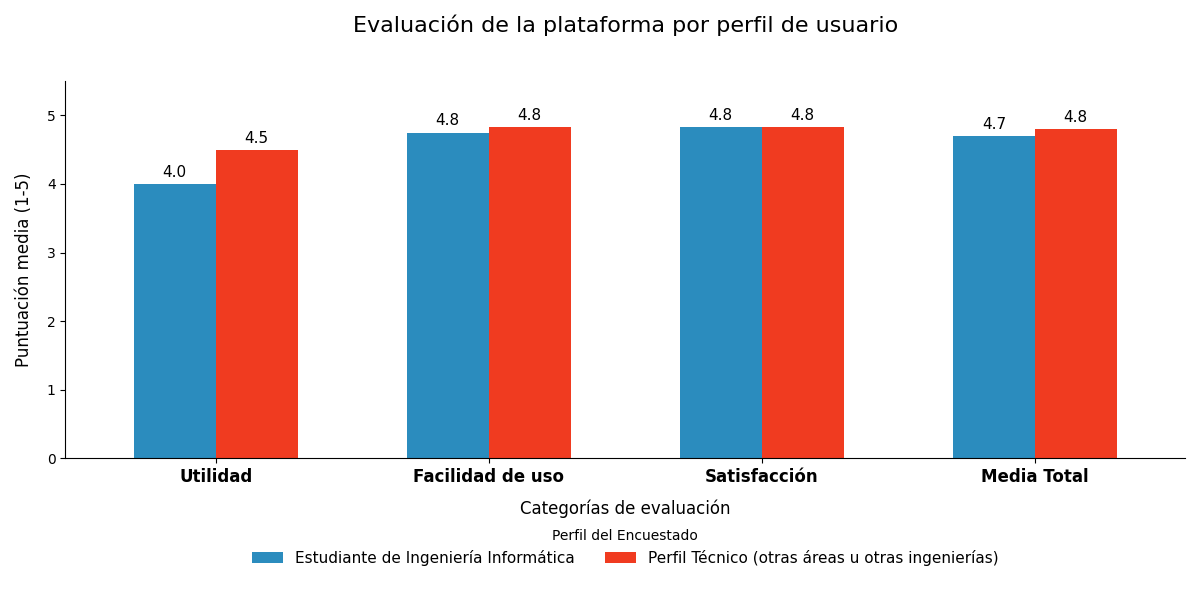
\includegraphics[width=0.95\textwidth]{./img/encuesta.png}
\end{figure}